\documentclass[tikz,border=10pt]{standalone}
\usepackage{tikz}
\usetikzlibrary{shapes.geometric, arrows.meta, positioning, backgrounds, shadows, patterns, decorations.pathmorphing, fit, calc}
\usepackage{xcolor}
\usepackage{amsmath}
\usepackage{booktabs}
\usepackage{array}
\usepackage{colortbl}

% Professional Color Scheme (matching Chapter 3)
\definecolor{primaryblue}{RGB}{41, 128, 185}
\definecolor{secondarygreen}{RGB}{39, 174, 96}
\definecolor{accentorange}{RGB}{230, 126, 34}
\definecolor{alertred}{RGB}{192, 57, 43}
\definecolor{purpleaccent}{RGB}{142, 68, 173}
\definecolor{tealaccent}{RGB}{22, 160, 133}
\definecolor{lightgray}{RGB}{236, 240, 241}
\definecolor{darkgray}{RGB}{52, 73, 94}
\definecolor{successgreen}{RGB}{39, 174, 96}
\definecolor{warningorange}{RGB}{243, 156, 18}

% TikZ Styles
\tikzset{
    % Timeline boxes
    phase box/.style={
        rectangle, rounded corners, draw=black, thick,
        minimum height=1.2cm, minimum width=3cm,
        text width=2.8cm, align=center, font=\small\sffamily\bfseries,
        drop shadow
    },
    % MAPE-K boxes
    mape box/.style={
        rectangle, rounded corners=5pt, draw=black, very thick,
        minimum height=2cm, minimum width=3.5cm,
        text width=3.2cm, align=center, font=\small\sffamily\bfseries,
        drop shadow={shadow xshift=2pt, shadow yshift=-2pt}
    },
    % Knowledge base (cylinder shape)
    knowledge/.style={
        cylinder, draw=black, very thick, aspect=0.3,
        minimum height=2.5cm, minimum width=3cm,
        shape border rotate=90, fill=warningorange!20,
        drop shadow, font=\small\sffamily\bfseries
    },
    % Arrows
    thick arrow/.style={
        -Stealth, very thick, color=darkgray
    },
    data arrow/.style={
        -Stealth, thick, color=primaryblue, dashed
    },
    % Downtime zone
    downtime zone/.style={
        rectangle, draw=alertred, very thick, dashed,
        fill=alertred!10, rounded corners
    },
    % Zero-downtime zone
    zero zone/.style={
        rectangle, draw=secondarygreen, very thick, dashed,
        fill=secondarygreen!10, rounded corners
    },
    % Annotation
    annotation/.style={
        rectangle, draw=darkgray, thick, rounded corners=3pt,
        fill=lightgray, text width=3cm, align=left, font=\footnotesize\sffamily
    }
}

\begin{document}

% ============================================================
% FIGURE 2.1: Reactive vs Proactive Recovery Timeline Comparison
% ============================================================
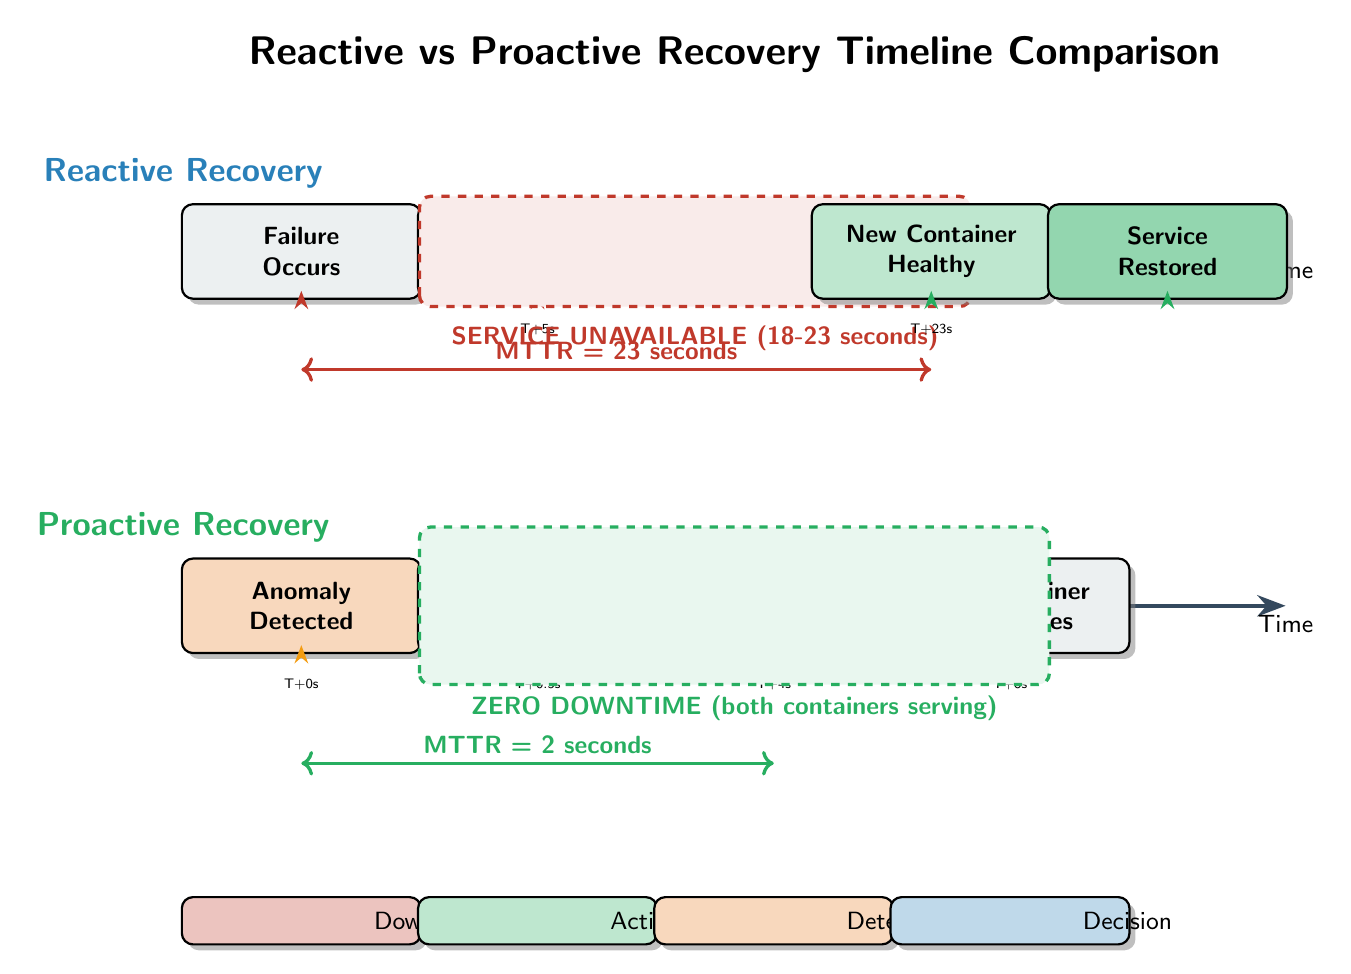
\begin{tikzpicture}[scale=1, every node/.style={transform shape}]

    % Title
    \node[font=\Large\sffamily\bfseries] at (7, 8.5) {Reactive vs Proactive Recovery Timeline Comparison};

    % ======== REACTIVE RECOVERY (TOP) ========
    \node[font=\large\sffamily\bfseries, primaryblue] at (0, 7) {Reactive Recovery};

    % Timeline arrow
    \draw[-Stealth, ultra thick, darkgray] (0, 6) -- (14, 6);
    \node[below, font=\small\sffamily] at (14, 6) {Time};

    % Events
    % T0: Failure occurs
    \node[phase box, fill=lightgray] (r1) at (1.5, 6) {Failure\\Occurs};
    \draw[-Stealth, thick, alertred] (r1.south) -- (1.5, 5.5);

    % T+5s: Health check detects
    \node[phase box, fill=accentorange!30] (r2) at (4.5, 6) {Health Check\\Detects};
    \draw[-Stealth, thick, alertred] (r2.south) -- (4.5, 5.5);
    \node[below, font=\tiny\sffamily] at (4.5, 5.2) {T+5s};

    % T+5-23s: DOWNTIME ZONE (red shaded)
    \draw[downtime zone] (3, 5.3) rectangle (10, 6.7);
    \node[font=\small\sffamily\bfseries, alertred] at (6.5, 4.9) {SERVICE UNAVAILABLE (18-23 seconds)};

    % T+23s: New container healthy
    \node[phase box, fill=secondarygreen!30] (r3) at (9.5, 6) {New Container\\Healthy};
    \draw[-Stealth, thick, secondarygreen] (r3.south) -- (9.5, 5.5);
    \node[below, font=\tiny\sffamily] at (9.5, 5.2) {T+23s};

    % T+23s+: Service restored
    \node[phase box, fill=secondarygreen!50] (r4) at (12.5, 6) {Service\\Restored};
    \draw[-Stealth, thick, secondarygreen] (r4.south) -- (12.5, 5.5);

    % MTTR annotation
    \draw[<->, very thick, alertred] (1.5, 4.5) -- (9.5, 4.5);
    \node[above, font=\small\sffamily\bfseries, alertred] at (5.5, 4.5) {MTTR = 23 seconds};

    % ======== PROACTIVE RECOVERY (BOTTOM) ========
    \node[font=\large\sffamily\bfseries, secondarygreen] at (0, 2.5) {Proactive Recovery};

    % Timeline arrow
    \draw[-Stealth, ultra thick, darkgray] (0, 1.5) -- (14, 1.5);
    \node[below, font=\small\sffamily] at (14, 1.5) {Time};

    % Events
    % T0: Anomaly detected
    \node[phase box, fill=accentorange!30] (p1) at (1.5, 1.5) {Anomaly\\Detected};
    \draw[-Stealth, thick, warningorange] (p1.south) -- (1.5, 1);
    \node[below, font=\tiny\sffamily] at (1.5, 0.7) {T+0s};

    % T+0.5s: Decision made
    \node[phase box, fill=primaryblue!30] (p2) at (4.5, 1.5) {Recovery\\Decision};
    \draw[-Stealth, thick, primaryblue] (p2.south) -- (4.5, 1);
    \node[below, font=\tiny\sffamily] at (4.5, 0.7) {T+0.5s};

    % T+4s: New container healthy
    \node[phase box, fill=secondarygreen!50] (p3) at (7.5, 1.5) {New Container\\Healthy};
    \draw[-Stealth, thick, secondarygreen] (p3.south) -- (7.5, 1);
    \node[below, font=\tiny\sffamily] at (7.5, 0.7) {T+4s};

    % T+8s: Old container terminates
    \node[phase box, fill=lightgray] (p4) at (10.5, 1.5) {Old Container\\Terminates};
    \draw[-Stealth, thick, darkgray] (p4.south) -- (10.5, 1);
    \node[below, font=\tiny\sffamily] at (10.5, 0.7) {T+8s};

    % ZERO-DOWNTIME ZONE (green shaded)
    \draw[zero zone] (3, 0.5) rectangle (11, 2.5);
    \node[font=\small\sffamily\bfseries, secondarygreen] at (7, 0.2) {ZERO DOWNTIME (both containers serving)};

    % MTTR annotation
    \draw[<->, very thick, secondarygreen] (1.5, -0.5) -- (7.5, -0.5);
    \node[above, font=\small\sffamily\bfseries, secondarygreen] at (4.5, -0.5) {MTTR = 2 seconds};

    % Legend
    \begin{scope}[shift={(0, -1.5)}]
        \node[phase box, fill=alertred!30, minimum width=1.5cm, minimum height=0.6cm] at (1.5, -1) {};
        \node[font=\small\sffamily, right] at (2.3, -1) {Downtime};

        \node[phase box, fill=secondarygreen!30, minimum width=1.5cm, minimum height=0.6cm] at (4.5, -1) {};
        \node[font=\small\sffamily, right] at (5.3, -1) {Active Service};

        \node[phase box, fill=accentorange!30, minimum width=1.5cm, minimum height=0.6cm] at (7.5, -1) {};
        \node[font=\small\sffamily, right] at (8.3, -1) {Detection};

        \node[phase box, fill=primaryblue!30, minimum width=1.5cm, minimum height=0.6cm] at (10.5, -1) {};
        \node[font=\small\sffamily, right] at (11.3, -1) {Decision};
    \end{scope}

\end{tikzpicture}

\newpage

% ============================================================
% FIGURE 2.2: MAPE-K Loop Applied to SwarmGuard
% ============================================================
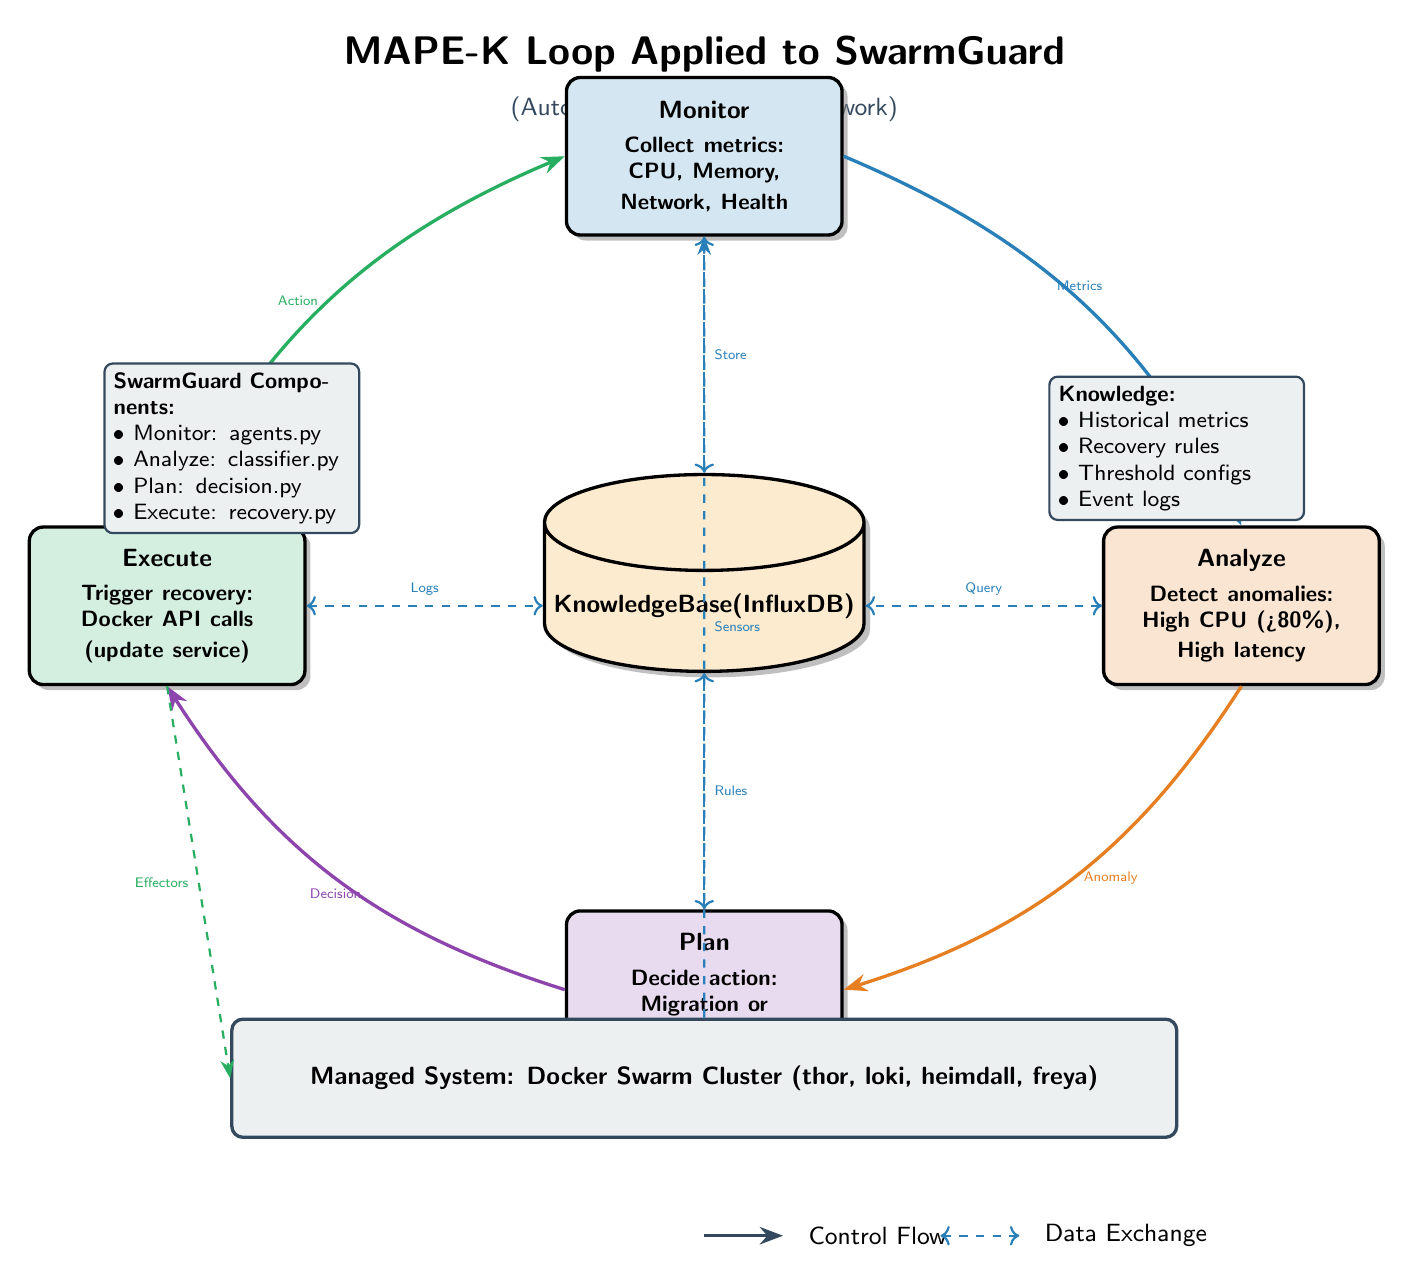
\begin{tikzpicture}[scale=1, every node/.style={transform shape}]

    % Title
    \node[font=\Large\sffamily\bfseries] at (0, 7) {MAPE-K Loop Applied to SwarmGuard};
    \node[font=\small\sffamily, darkgray] at (0, 6.3) {(Autonomic Computing Framework)};

    % Center: Knowledge Base (cylinder)
    \node[knowledge] (K) at (0, 0) {Knowledge\\Base\\(InfluxDB)};

    % Top: Monitor
    \node[mape box, fill=primaryblue!20, above=3cm of K] (M) {
        \textbf{Monitor}\\[3pt]
        \footnotesize Collect metrics:\\
        CPU, Memory,\\
        Network, Health
    };

    % Right: Analyze
    \node[mape box, fill=accentorange!20, right=3cm of K] (A) {
        \textbf{Analyze}\\[3pt]
        \footnotesize Detect anomalies:\\
        High CPU (>80\%),\\
        High latency
    };

    % Bottom: Plan
    \node[mape box, fill=purpleaccent!20, below=3cm of K] (P) {
        \textbf{Plan}\\[3pt]
        \footnotesize Decide action:\\
        Migration or\\
        Scaling
    };

    % Left: Execute
    \node[mape box, fill=secondarygreen!20, left=3cm of K] (E) {
        \textbf{Execute}\\[3pt]
        \footnotesize Trigger recovery:\\
        Docker API calls\\
        (update service)
    };

    % Circular flow arrows (CLOCKWISE: M -> A -> P -> E -> M)
    \draw[thick arrow, primaryblue] (M.east) to[bend left=20] node[midway, above, font=\tiny\sffamily] {Metrics} (A.north);
    \draw[thick arrow, accentorange] (A.south) to[bend left=20] node[midway, right, font=\tiny\sffamily] {Anomaly} (P.east);
    \draw[thick arrow, purpleaccent] (P.west) to[bend left=20] node[midway, below, font=\tiny\sffamily] {Decision} (E.south);
    \draw[thick arrow, secondarygreen] (E.north) to[bend left=20] node[midway, left, font=\tiny\sffamily] {Action} (M.west);

    % Knowledge Base connections (bidirectional dashed)
    \draw[data arrow, <->] (M.south) -- (K.north) node[midway, right, font=\tiny\sffamily] {Store};
    \draw[data arrow, <->] (A.west) -- (K.east) node[midway, above, font=\tiny\sffamily] {Query};
    \draw[data arrow, <->] (P.north) -- (K.south) node[midway, right, font=\tiny\sffamily] {Rules};
    \draw[data arrow, <->] (E.east) -- (K.west) node[midway, above, font=\tiny\sffamily] {Logs};

    % Managed System (external)
    \node[rectangle, draw=darkgray, very thick, rounded corners, fill=lightgray,
          minimum width=12cm, minimum height=1.5cm, font=\small\sffamily\bfseries] (Sys) at (0, -6) {
        Managed System: Docker Swarm Cluster (thor, loki, heimdall, freya)
    };

    % Sensors and Effectors
    \draw[-Stealth, thick, primaryblue, dashed] (Sys.north) -- (M.south) node[midway, right, font=\tiny\sffamily] {Sensors};
    \draw[-Stealth, thick, secondarygreen, dashed] (E.south) -- (Sys.west) node[midway, left, font=\tiny\sffamily] {Effectors};

    % Annotations
    \node[annotation] at (-6, 2) {
        \textbf{SwarmGuard Components:}\\
        • Monitor: agents.py\\
        • Analyze: classifier.py\\
        • Plan: decision.py\\
        • Execute: recovery.py
    };

    \node[annotation] at (6, 2) {
        \textbf{Knowledge:}\\
        • Historical metrics\\
        • Recovery rules\\
        • Threshold configs\\
        • Event logs
    };

    % Legend
    \begin{scope}[shift={(0, -8)}]
        \draw[thick arrow] (0, 0) -- (1, 0);
        \node[right, font=\small\sffamily] at (1.2, 0) {Control Flow};

        \draw[data arrow, <->] (3, 0) -- (4, 0);
        \node[right, font=\small\sffamily] at (4.2, 0) {Data Exchange};
    \end{scope}

\end{tikzpicture}

\newpage

% ============================================================
% TABLE 2.1: Docker Swarm vs Kubernetes Feature Comparison
% ============================================================
\begin{tikzpicture}
    \node[font=\Large\sffamily\bfseries] at (0, 1) {Table 2.1: Docker Swarm vs Kubernetes Feature Comparison};

    \node at (0, -4) {
        \begin{tabular}{@{}p{4.5cm}p{4.5cm}p{4.5cm}@{}}
            \toprule
            \textbf{Feature} & \textbf{Docker Swarm} & \textbf{Kubernetes} \\
            \midrule
            \rowcolor{lightgray}
            \textbf{Learning Curve} & Simple, easy to learn & Steep, complex \\
            \textbf{Setup Complexity} & Minimal (built into Docker) & Requires multiple components \\
            \rowcolor{lightgray}
            \textbf{Deployment Speed} & Fast (seconds) & Slower (minutes) \\
            \textbf{Scalability} & Good (up to 100s nodes) & Excellent (1000s nodes) \\
            \rowcolor{lightgray}
            \textbf{Health Checks} & HTTP, TCP, Command & HTTP, TCP, gRPC, Command \\
            \textbf{Rolling Updates} & ✅ Built-in & ✅ Built-in \\
            \rowcolor{lightgray}
            \textbf{Auto-Scaling} & ❌ Manual only & ✅ HPA, VPA, Cluster AS \\
            \textbf{Load Balancing} & ✅ Routing mesh & ✅ Services, Ingress \\
            \rowcolor{lightgray}
            \textbf{Self-Healing} & ✅ Reactive (restart) & ✅ Reactive (restart) \\
            \textbf{Proactive Recovery} & ❌ None & ❌ None (research area) \\
            \rowcolor{lightgray}
            \textbf{Community Size} & Smaller, declining & Very large, growing \\
            \textbf{Best Use Case} & Small-medium apps, simplicity & Large-scale, enterprise \\
            \rowcolor{lightgray}
            \textbf{Industry Adoption} & ~5-10\% & ~85-90\% \\
            \bottomrule
        \end{tabular}
    };

    \node[font=\small\sffamily, text width=12cm, align=left] at (0, -10.5) {
        \textbf{Key Insight:} Both platforms lack \textit{proactive} recovery mechanisms out-of-the-box. \\
        SwarmGuard addresses this gap specifically for Docker Swarm users who prioritize simplicity.
    };
\end{tikzpicture}

\newpage

% ============================================================
% TABLE 2.2: Comparative Analysis - Related Work
% ============================================================
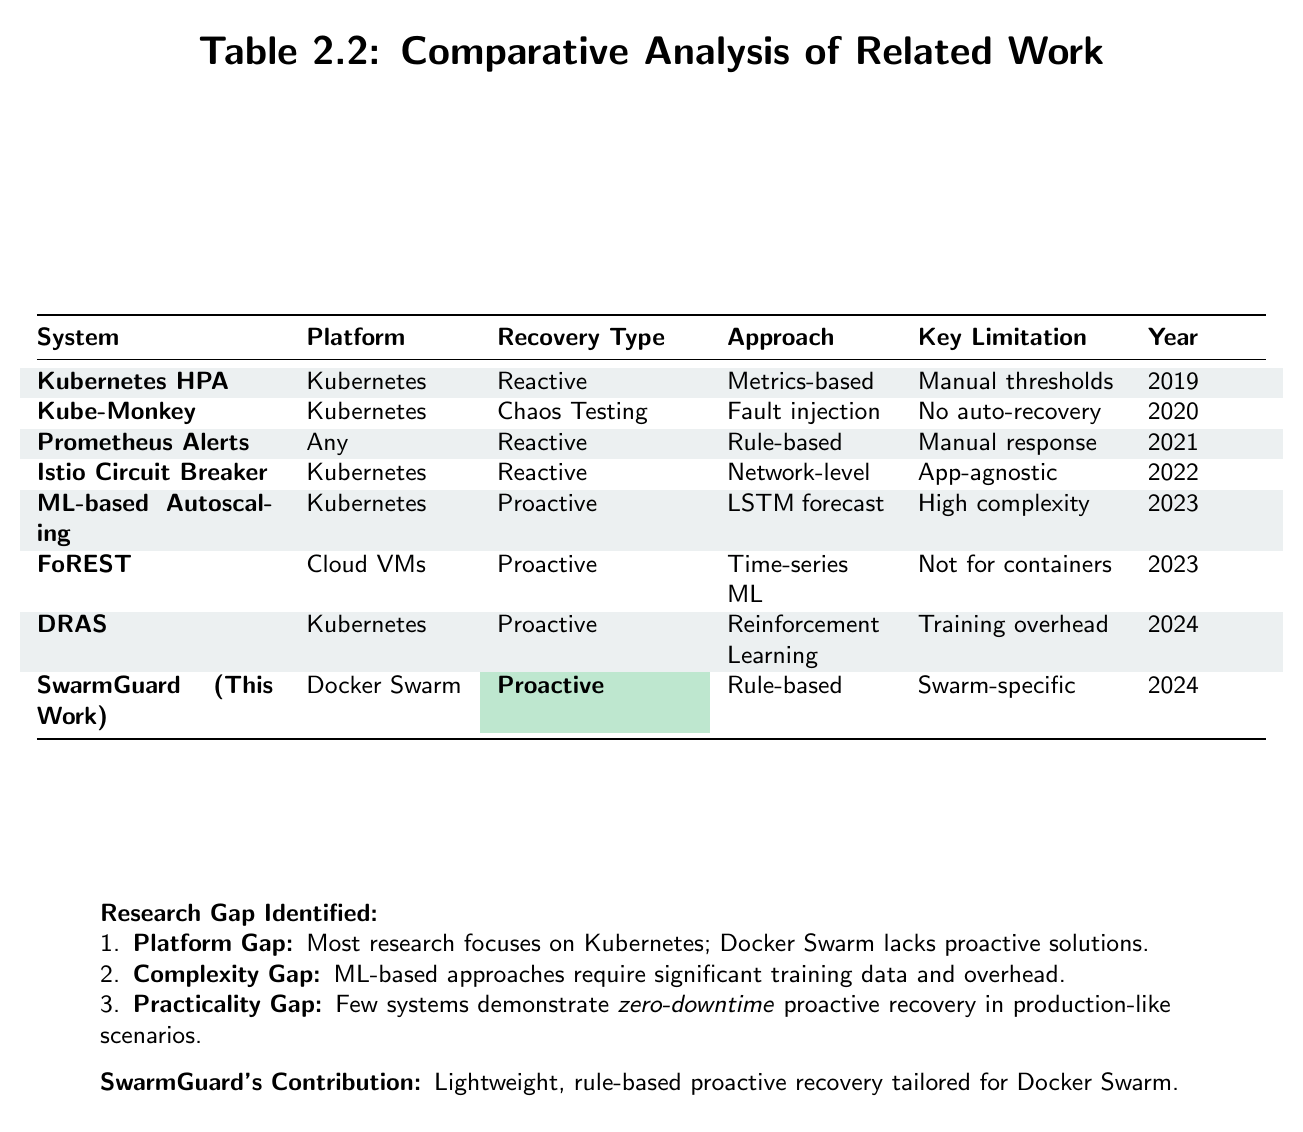
\begin{tikzpicture}
    \node[font=\Large\sffamily\bfseries] at (0, 1) {Table 2.2: Comparative Analysis of Related Work};

    \node at (0, -5) {
        \small\sffamily
        \begin{tabular}{@{}p{3cm}p{2cm}p{2.5cm}p{2cm}p{2.5cm}p{1.5cm}@{}}
            \toprule
            \textbf{System} & \textbf{Platform} & \textbf{Recovery Type} & \textbf{Approach} & \textbf{Key Limitation} & \textbf{Year} \\
            \midrule
            \rowcolor{lightgray}
            \textbf{Kubernetes HPA} & Kubernetes & Reactive & Metrics-based & Manual thresholds & 2019 \\
            \textbf{Kube-Monkey} & Kubernetes & Chaos Testing & Fault injection & No auto-recovery & 2020 \\
            \rowcolor{lightgray}
            \textbf{Prometheus Alerts} & Any & Reactive & Rule-based & Manual response & 2021 \\
            \textbf{Istio Circuit Breaker} & Kubernetes & Reactive & Network-level & App-agnostic & 2022 \\
            \rowcolor{lightgray}
            \textbf{ML-based Autoscaling} & Kubernetes & Proactive & LSTM forecast & High complexity & 2023 \\
            \textbf{FoREST} & Cloud VMs & Proactive & Time-series ML & Not for containers & 2023 \\
            \rowcolor{lightgray}
            \textbf{DRAS} & Kubernetes & Proactive & Reinforcement Learning & Training overhead & 2024 \\
            \textbf{SwarmGuard (This Work)} & Docker Swarm & \cellcolor{secondarygreen!30}\textbf{Proactive} & Rule-based & Swarm-specific & 2024 \\
            \bottomrule
        \end{tabular}
    };

    \node[font=\small\sffamily, text width=14cm, align=left] at (0, -11) {
        \textbf{Research Gap Identified:}\\
        1. \textbf{Platform Gap:} Most research focuses on Kubernetes; Docker Swarm lacks proactive solutions.\\
        2. \textbf{Complexity Gap:} ML-based approaches require significant training data and overhead.\\
        3. \textbf{Practicality Gap:} Few systems demonstrate \textit{zero-downtime} proactive recovery in production-like scenarios.\\[6pt]
        \textbf{SwarmGuard's Contribution:} Lightweight, rule-based proactive recovery tailored for Docker Swarm.
    };
\end{tikzpicture}

\end{document}
